\documentclass{scrartcl}			% defines the kind of document you want to produce

% Include different packages:
\usepackage[utf8]{inputenc}
\usepackage[T1]{fontenc}
\usepackage{lmodern}
\usepackage[english]{babel}
\usepackage{amsmath}
\usepackage{float}
\usepackage{graphicx}           	% include graphics
\usepackage{caption}
\usepackage{subcaption}
\usepackage{hyperref}
\usepackage{listings}

\title{Neuroprothetik Exercise 2}
\author{Aleksandra Teska}
\date{12. May 2018}


\begin{document} 					% Document begins here

\maketitle

\section{Plot slope fields and isocline}		% start a new section
The goal of this exercise was to plot the slope fields for $t \in [−5, 5 ]s$ and $V \in [−5, 5 ]V$ as well as the isocline for (-2, -1, 0, 1, 2) $\frac{V}{s}$, for the following differential equations.

\begin{align}
\frac{dV}{dt} =  1 - V -t
\end{align}			
\begin{align}
\frac{dV}{dt} = \sin(t) - \frac{1}{1.5}V
\end{align}			

%\subsection{Plots of slope fields of differential equations}		% start a new section
\begin{figure}[H]					%start figure-environment
	\centering
	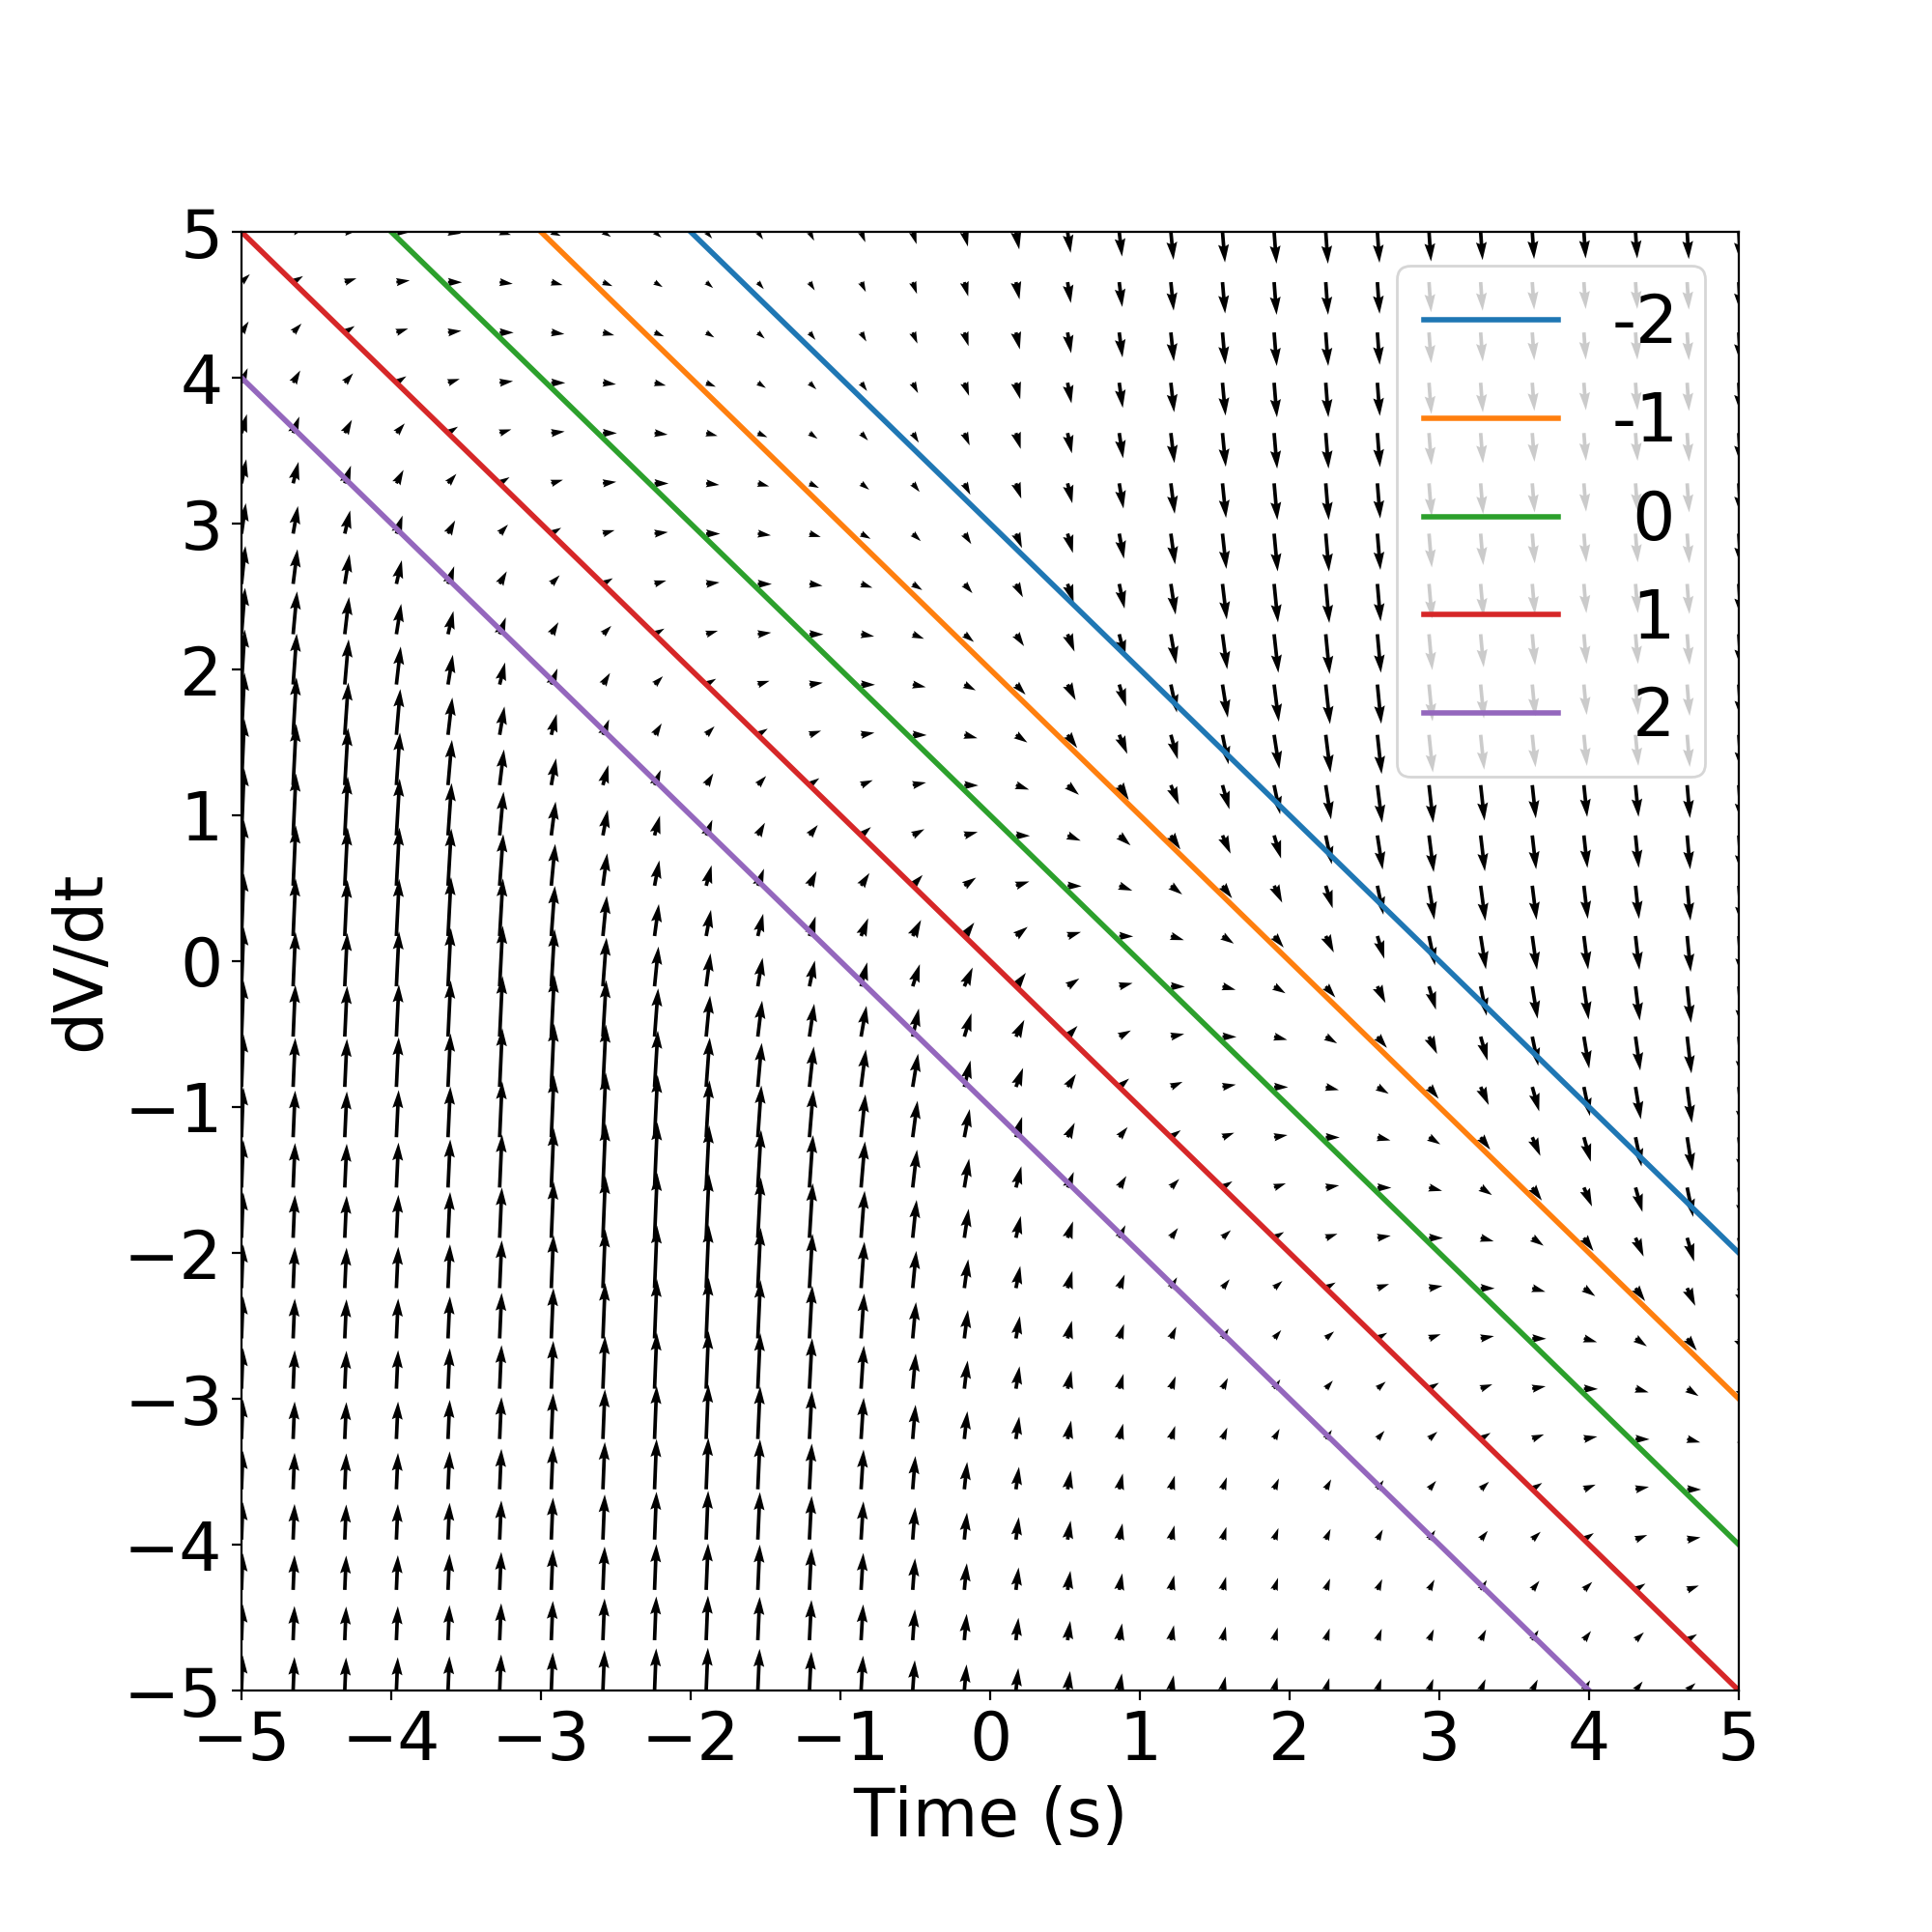
\includegraphics[scale=0.36]{1_0.png}
	\captionsetup{width=\linewidth}  %choose the with of the caption
	\caption{Slope field and isoclines for equation (1)}
	\label{subsec_fig1_0} %choose a label, see subsection references
\end{figure}

\begin{figure}[H]					%start figure-environment
	\centering
	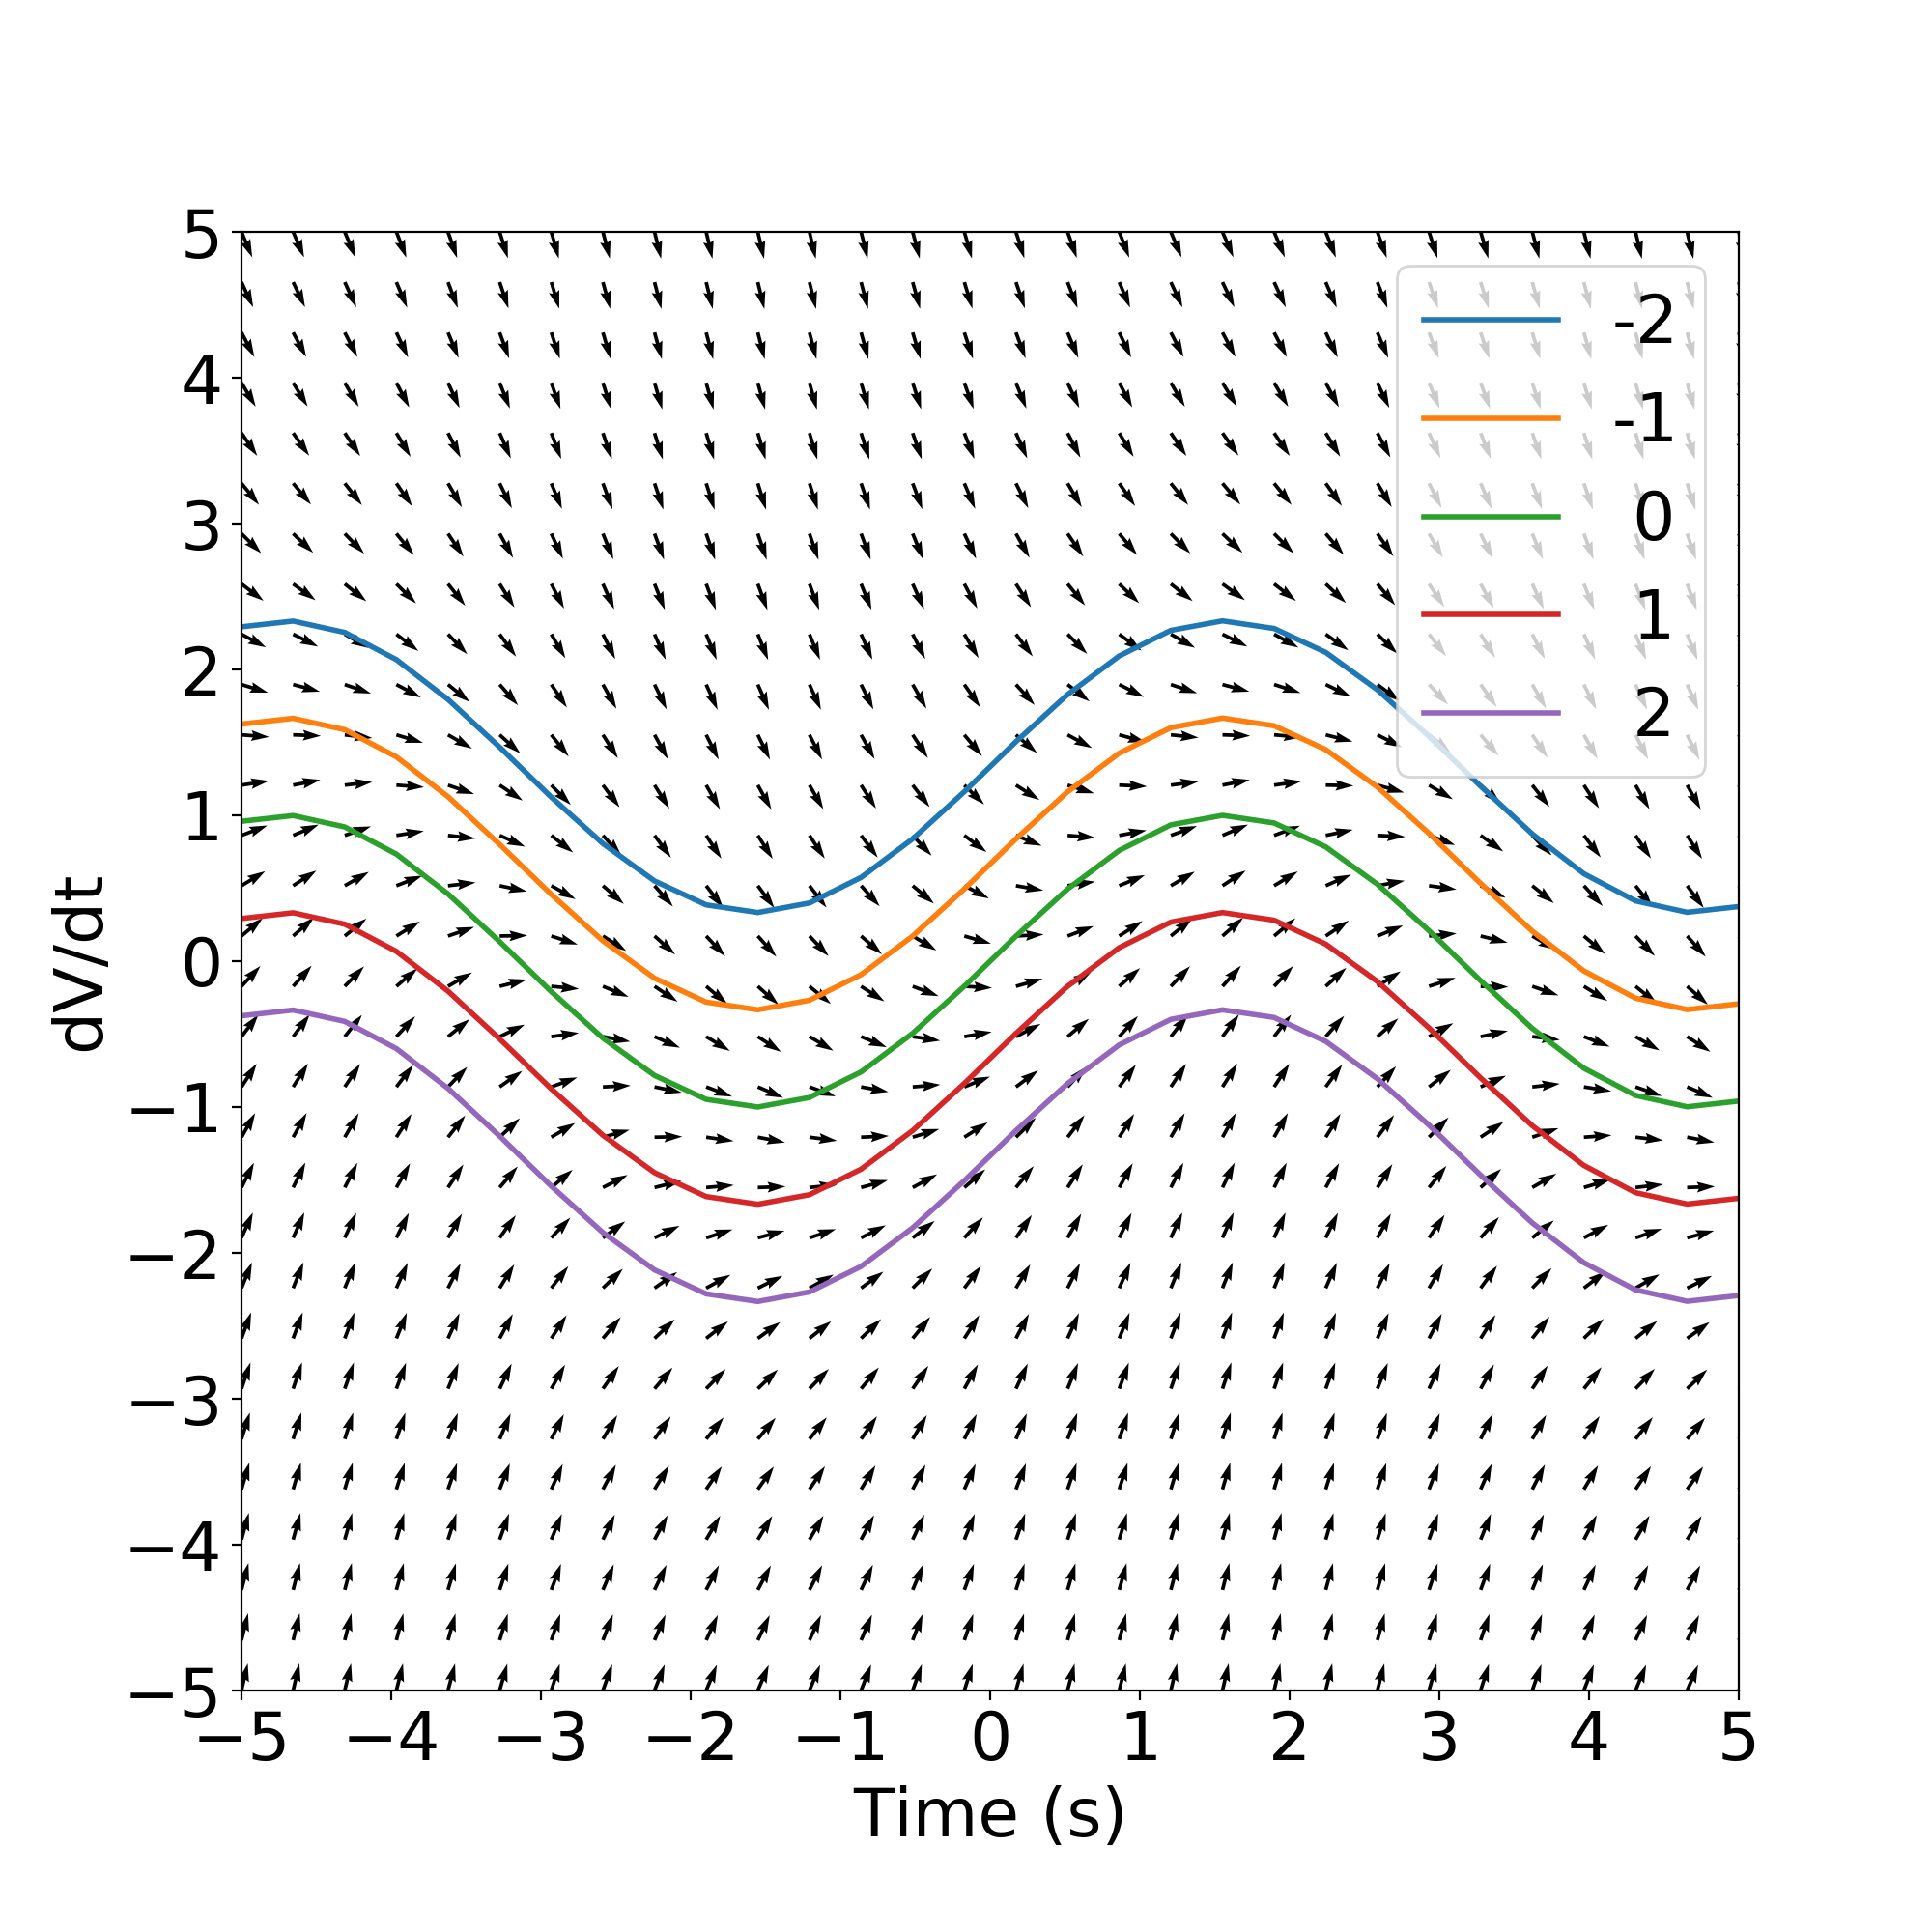
\includegraphics[scale=0.36]{1_1.png}
	\captionsetup{width=\linewidth}  %choose the with of the caption
	\caption{Slope field and isoclines for equation (2)}
	\label{subsec_fig1_1} %choose a label, see subsection references
\end{figure}

\section{Differential equations of a simple cell model}

Derivation of the differential equation for the following equivalent circuit of a leaky integrate
and fire neuron. Following implementation was used to solve the exercise:
\begin{verbatim}
I_calD = lambda t, Imax: Imax * np.sin(t) + D 
ode_rhs_cell = lambda V, I: (-V + R * I)/ R * C
\end{verbatim}


\begin{figure}[H]					%start figure-environment
	\centering
	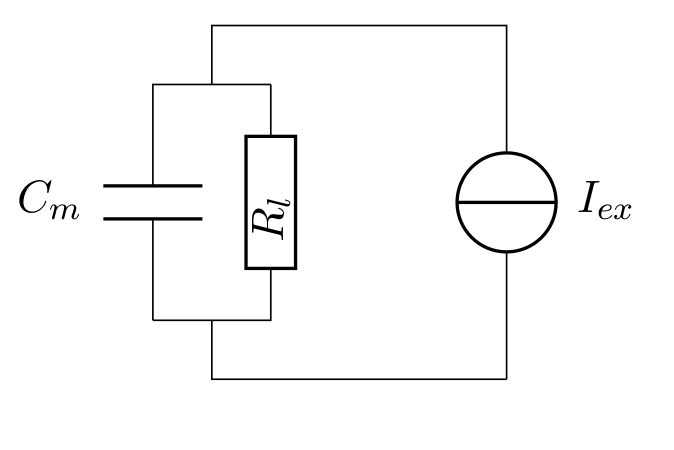
\includegraphics[scale=0.3]{1.png}
	\captionsetup{width=\linewidth}  %choose the with of the caption
	\caption{Equivalent circuit of a leaky integrate and fire neuron}
	\label{subsec_fig} %choose a label, see subsection references
\end{figure}
%Figure \ref{subsec_fig}
\begin{align}
I_{max} = I_{ex} \sin(t)
\end{align}			


\subsection{Plot the slope field}
Plots of the slope field for:
\begin{itemize}
	\item $R_{l}$ = 1 $\Omega$; C=1 F; $I_{max}$=0 A
	\item $R_{l}$ = 1 $\Omega$; C=1 F; $I_{max}$=1 A
\end{itemize}
Add another constant term D=2 A to the differential equation and plot:	
\begin{itemize}
	\item $R_{l}$ = 1 $\Omega$; C=1 F; $I_{max}$=0 A
	\item $R_{l}$ = 1 $\Omega$; C=1 F; $I_{max}$=1 A
\end{itemize}

\begin{figure*}[h]					%start figure-environment
	\centering
	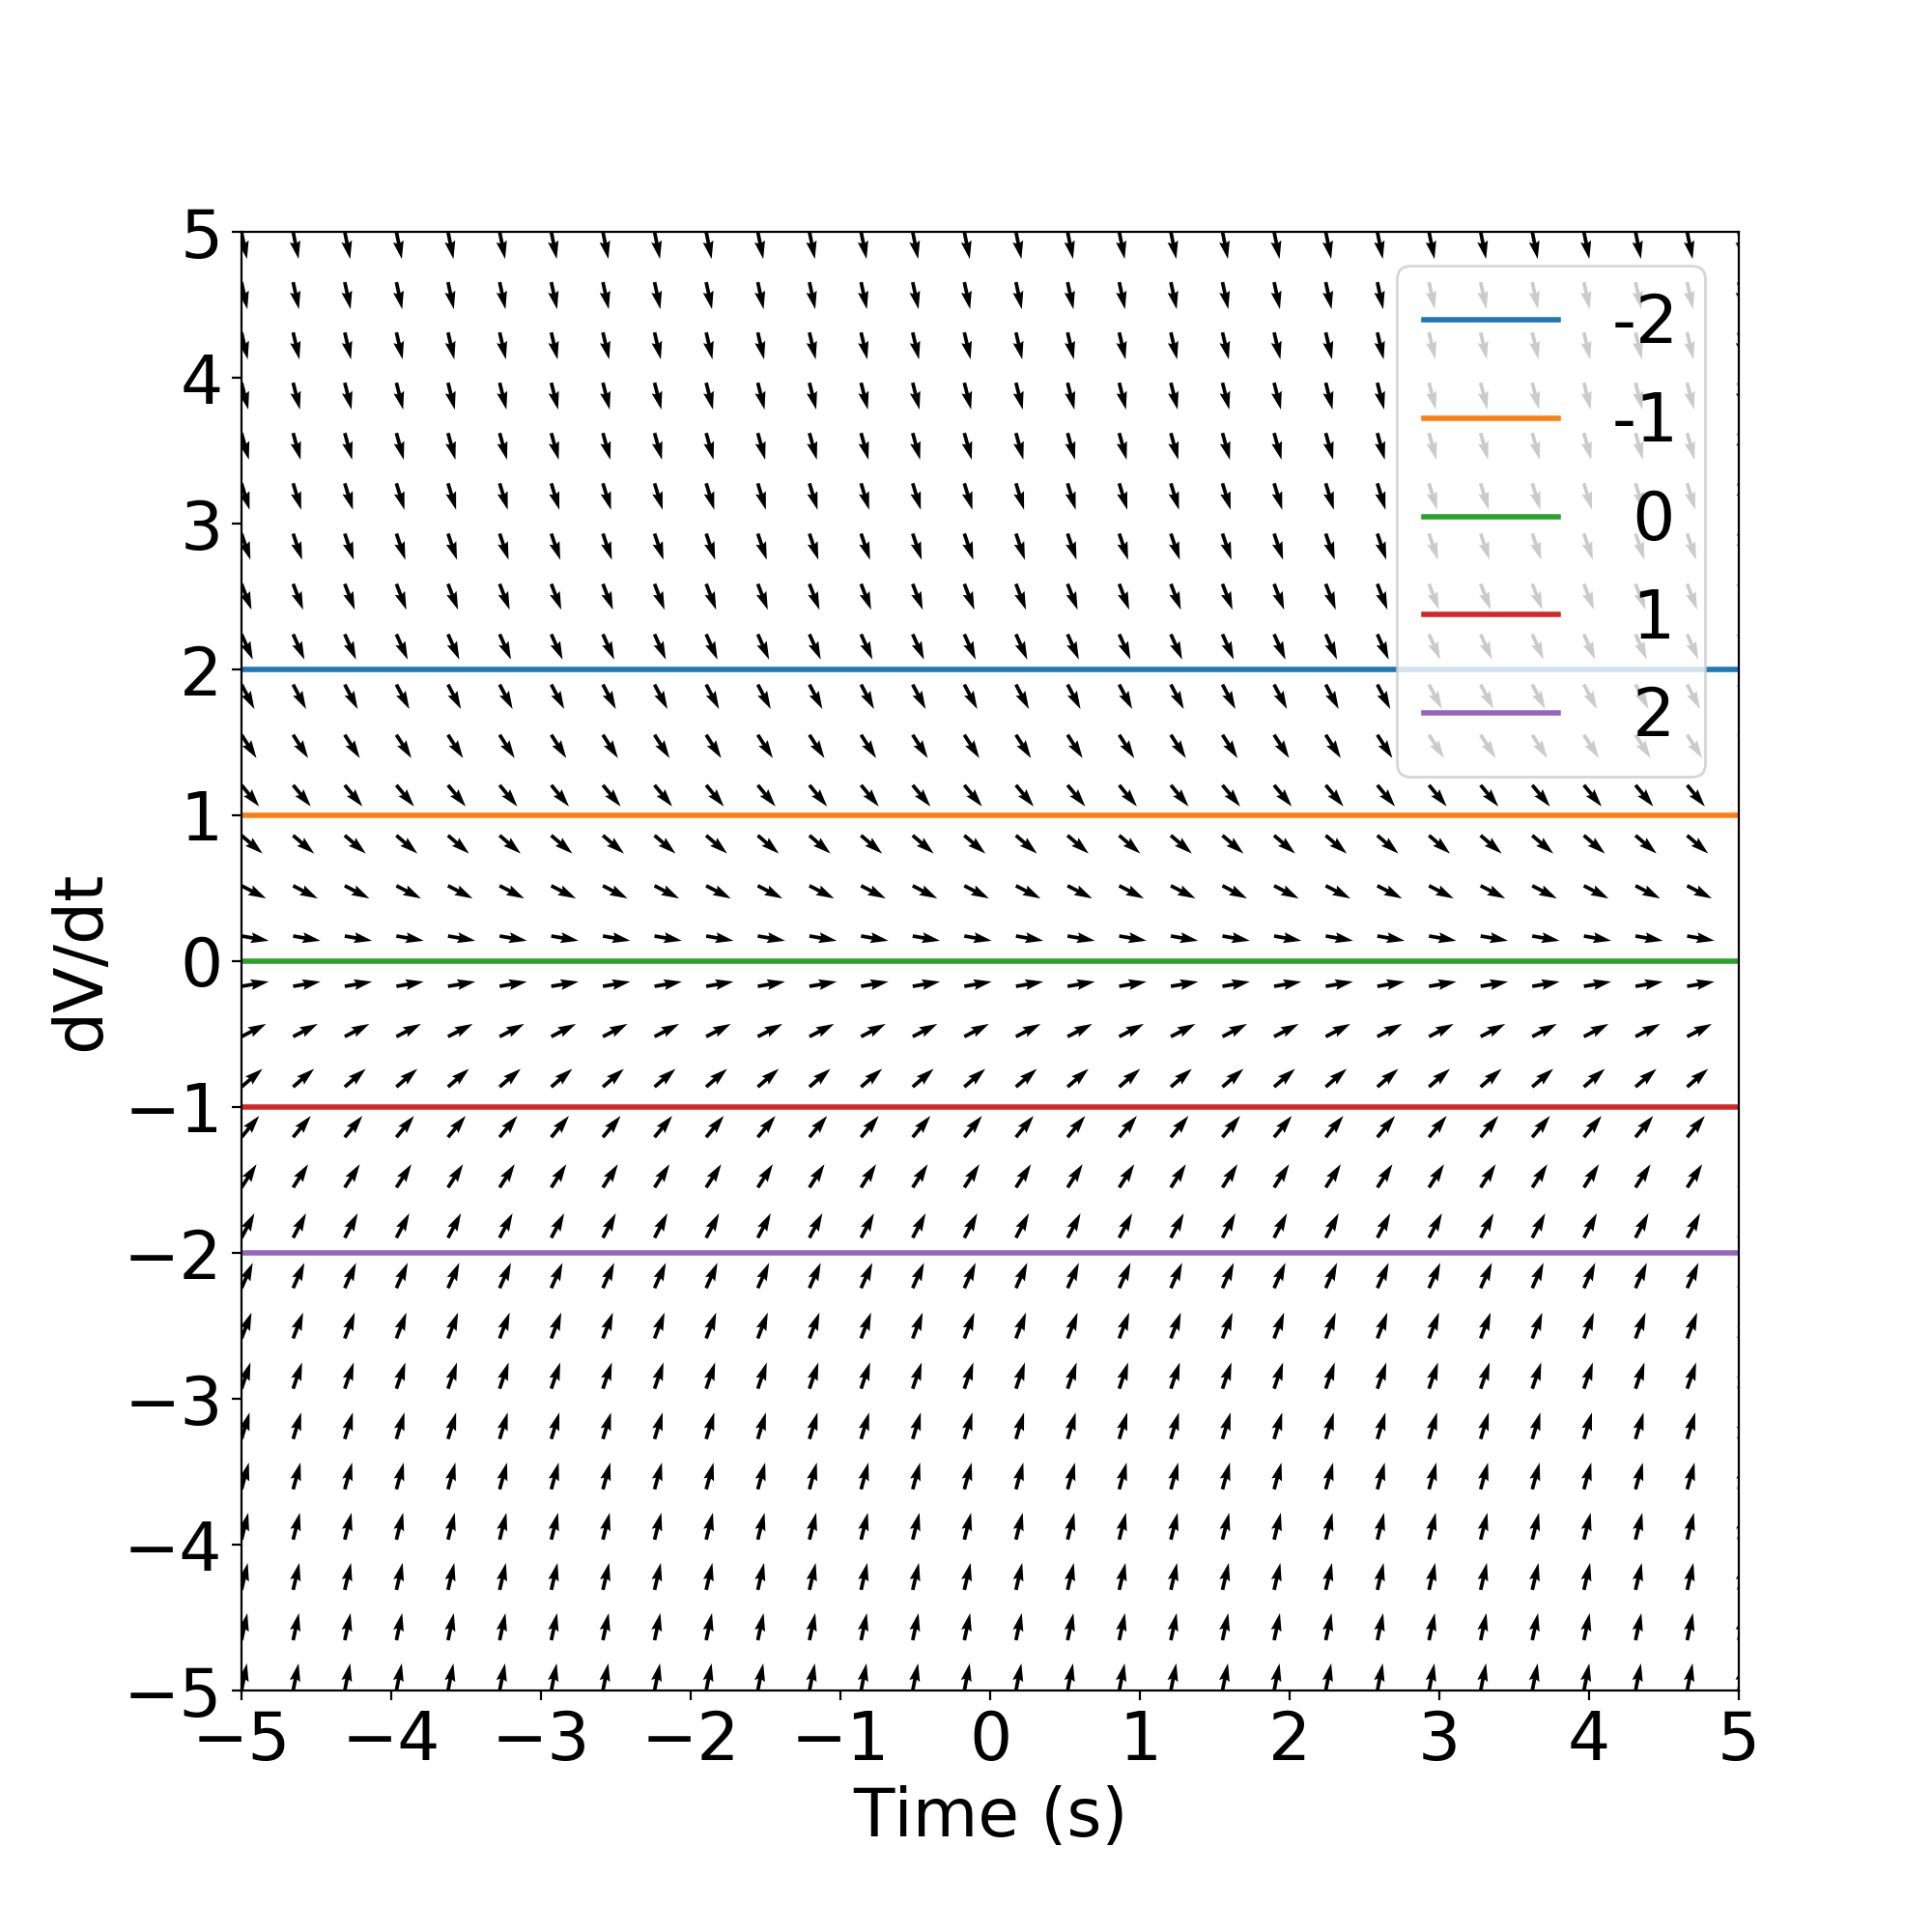
\includegraphics[scale=0.36]{2_0.png}
	\captionsetup{width=\linewidth}  %choose the with of the caption
	\caption{Slope field and isoclines for simple cell model, $R_{l}$ = 1 $\Omega$; C=1 F; $I_{max}$=0 A}
	\label{subsec_fig2_0} %choose a label, see subsection references
\end{figure*}

\begin{figure*}[h]					%start figure-environment
	\centering
	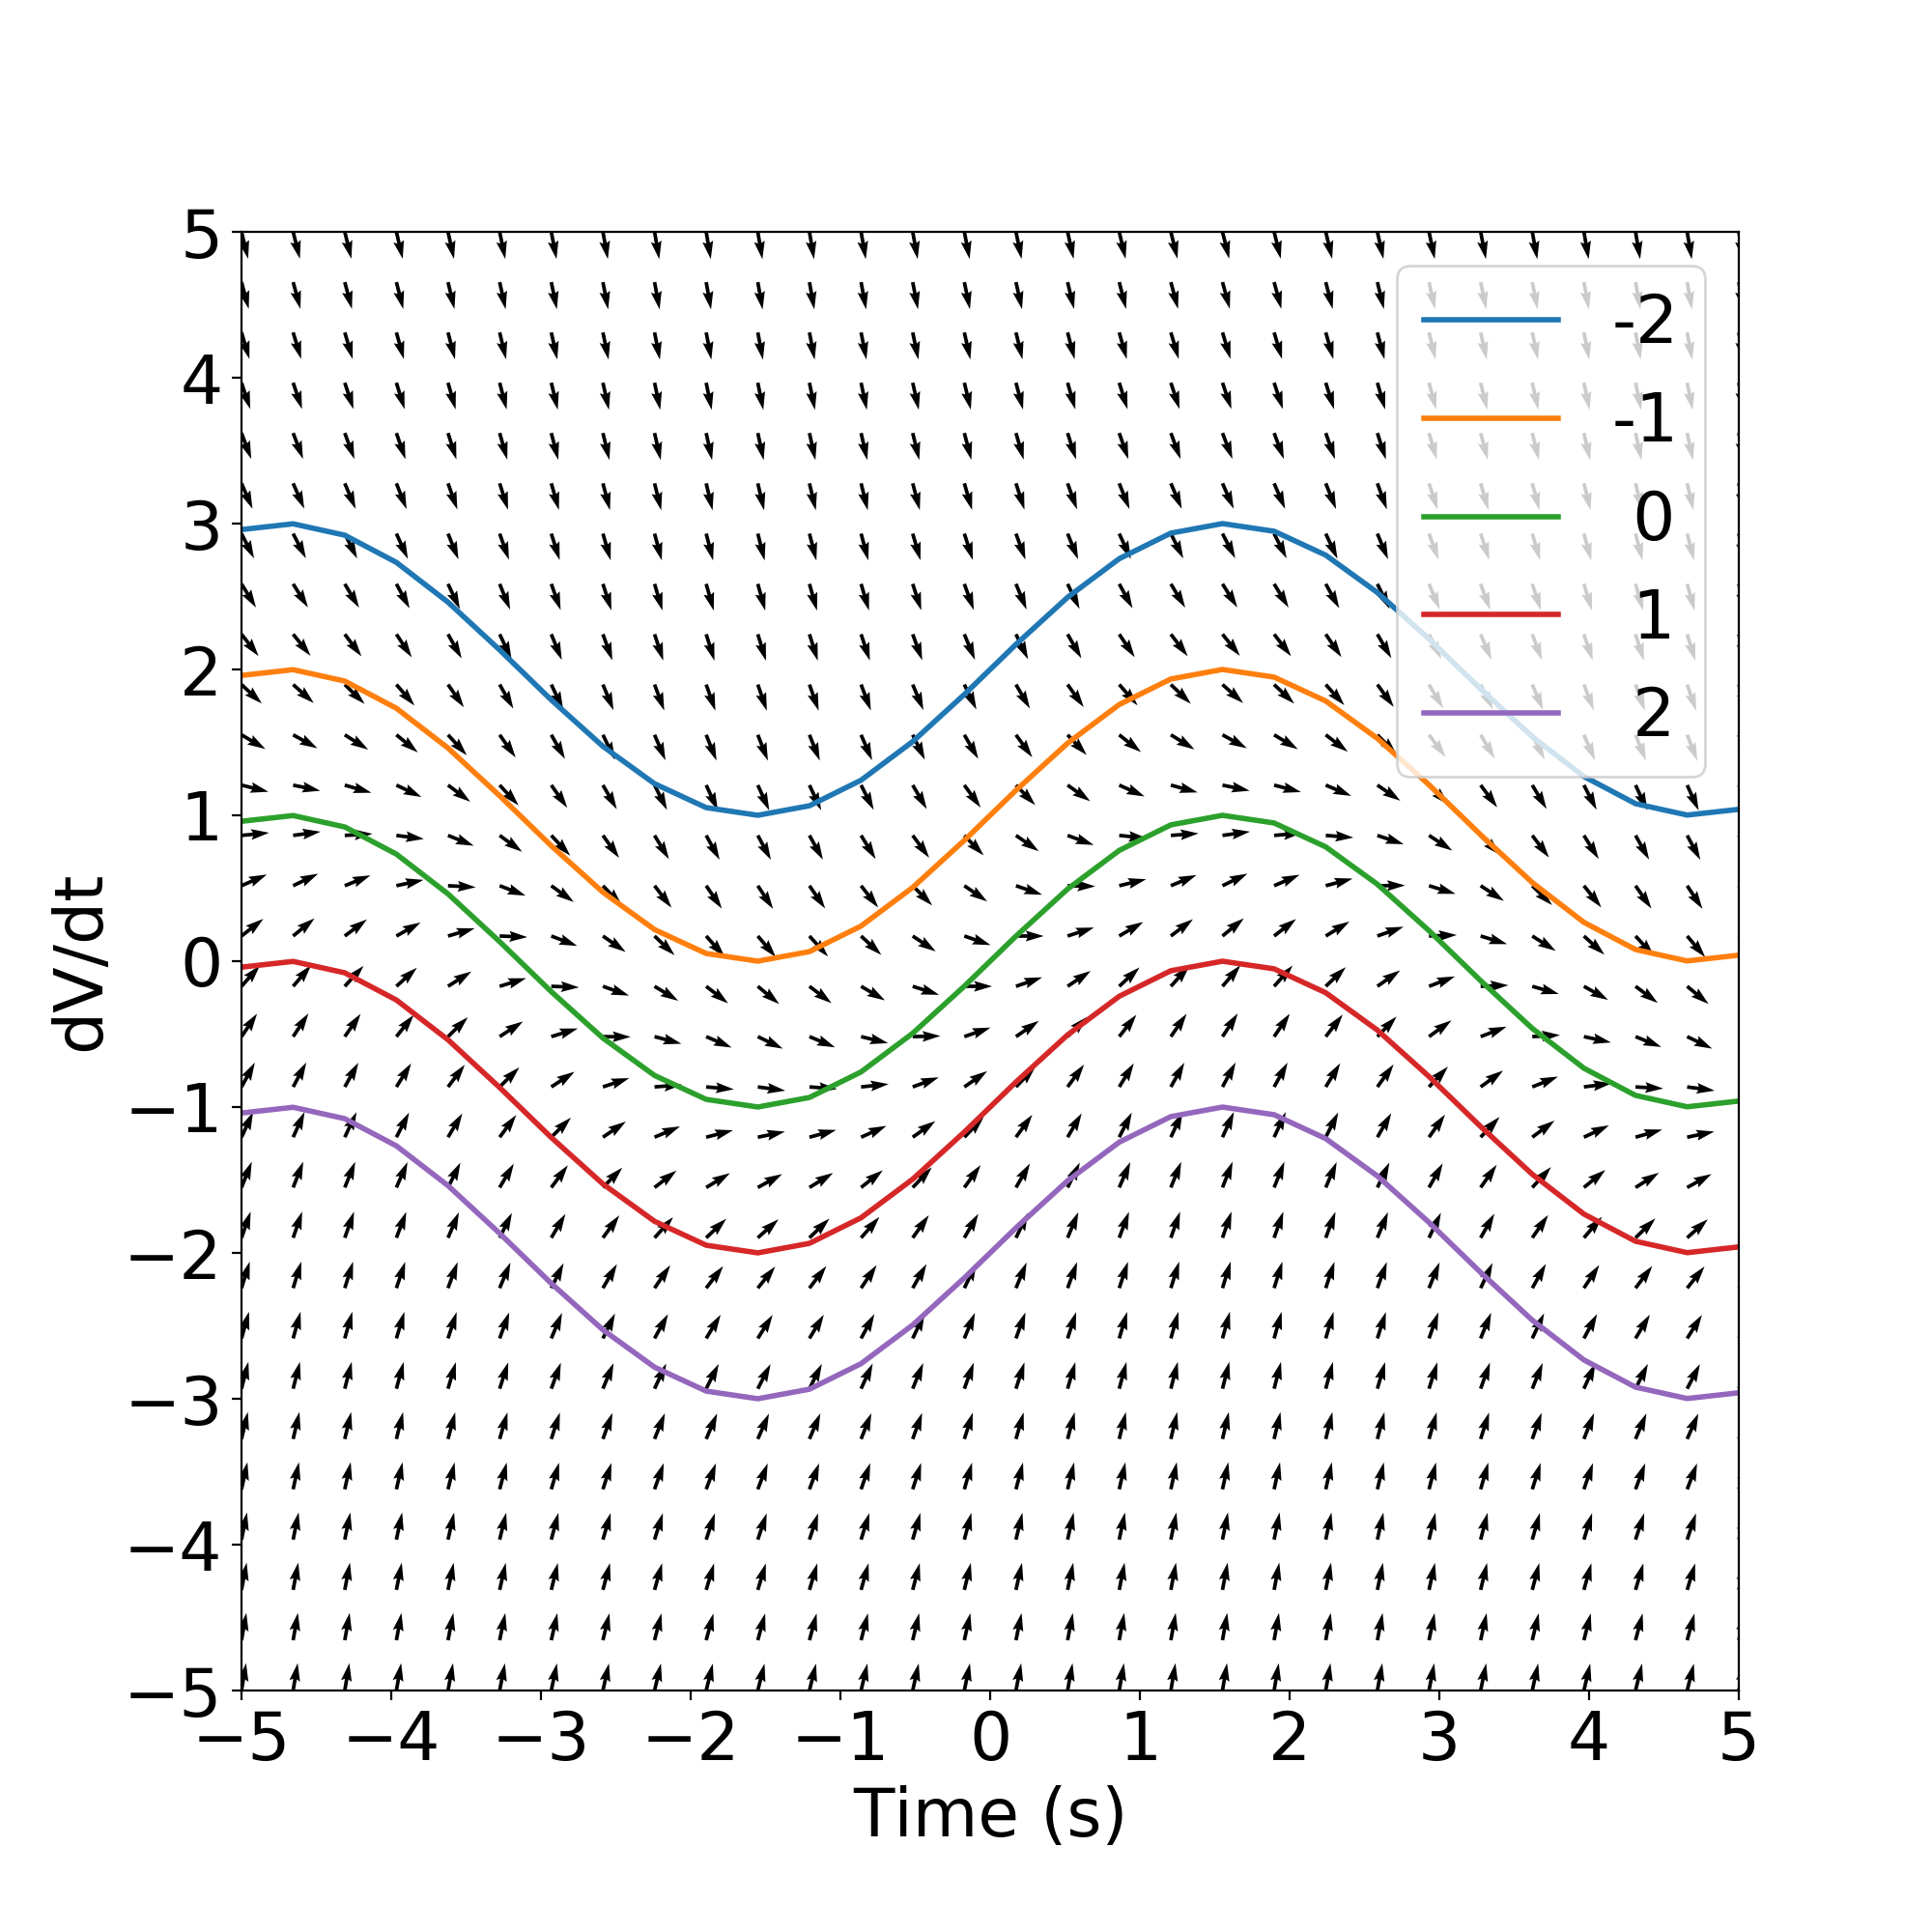
\includegraphics[scale=0.36]{2_1.png}
	\captionsetup{width=\linewidth}  %choose the with of the caption
	\caption{Slope field and isoclines for simple cell model, $R_{l}$ = 1 $\Omega$; C=1 F; $I_{max}$=1 A}
	\label{subsec_fig2_1} %choose a label, see subsection references
\end{figure*}

\begin{figure*}[h]					%start figure-environment
	\centering
	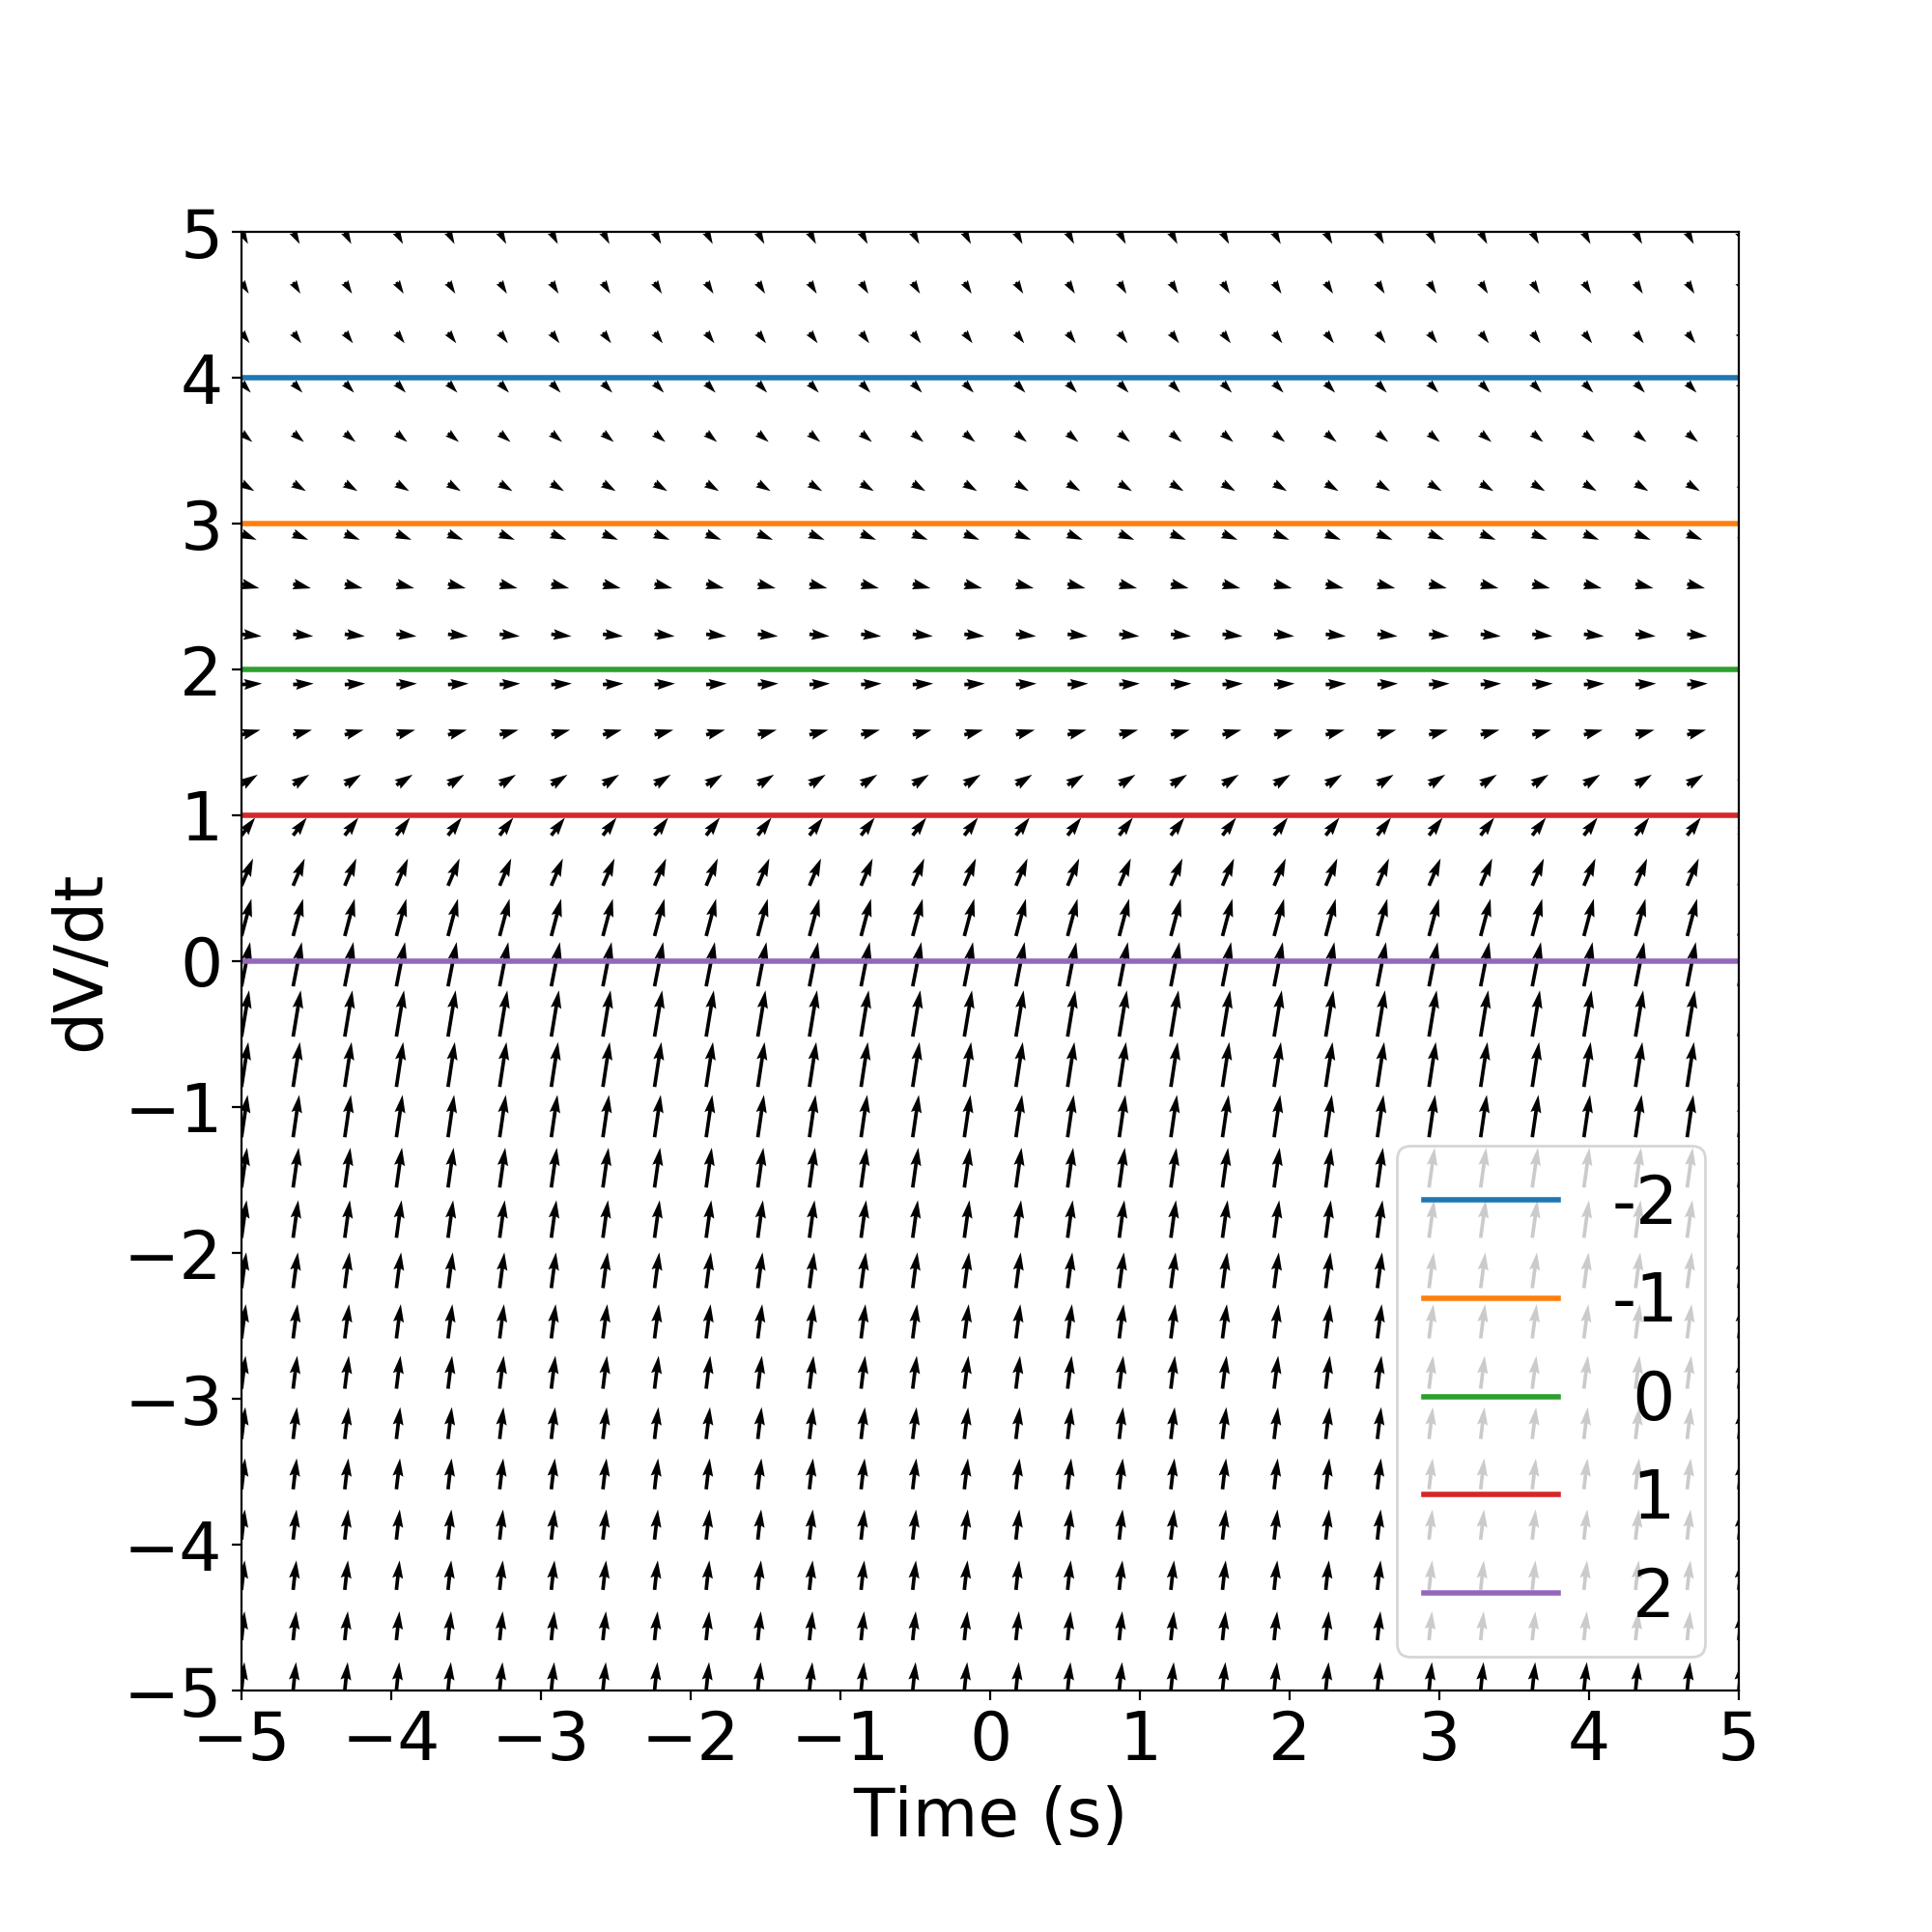
\includegraphics[scale=0.36]{2_2.png}
	\captionsetup{width=\linewidth}  %choose the with of the caption
	\caption{Slope field and isoclines for simple cell model, $R_{l}$ = 1 $\Omega$; C=1 F; $I_{max}$=0 A, D=2A}
	\label{subsec_fig2_2} %choose a label, see subsection references
\end{figure*}

\begin{figure*}[h]					%start figure-environment
	\centering
	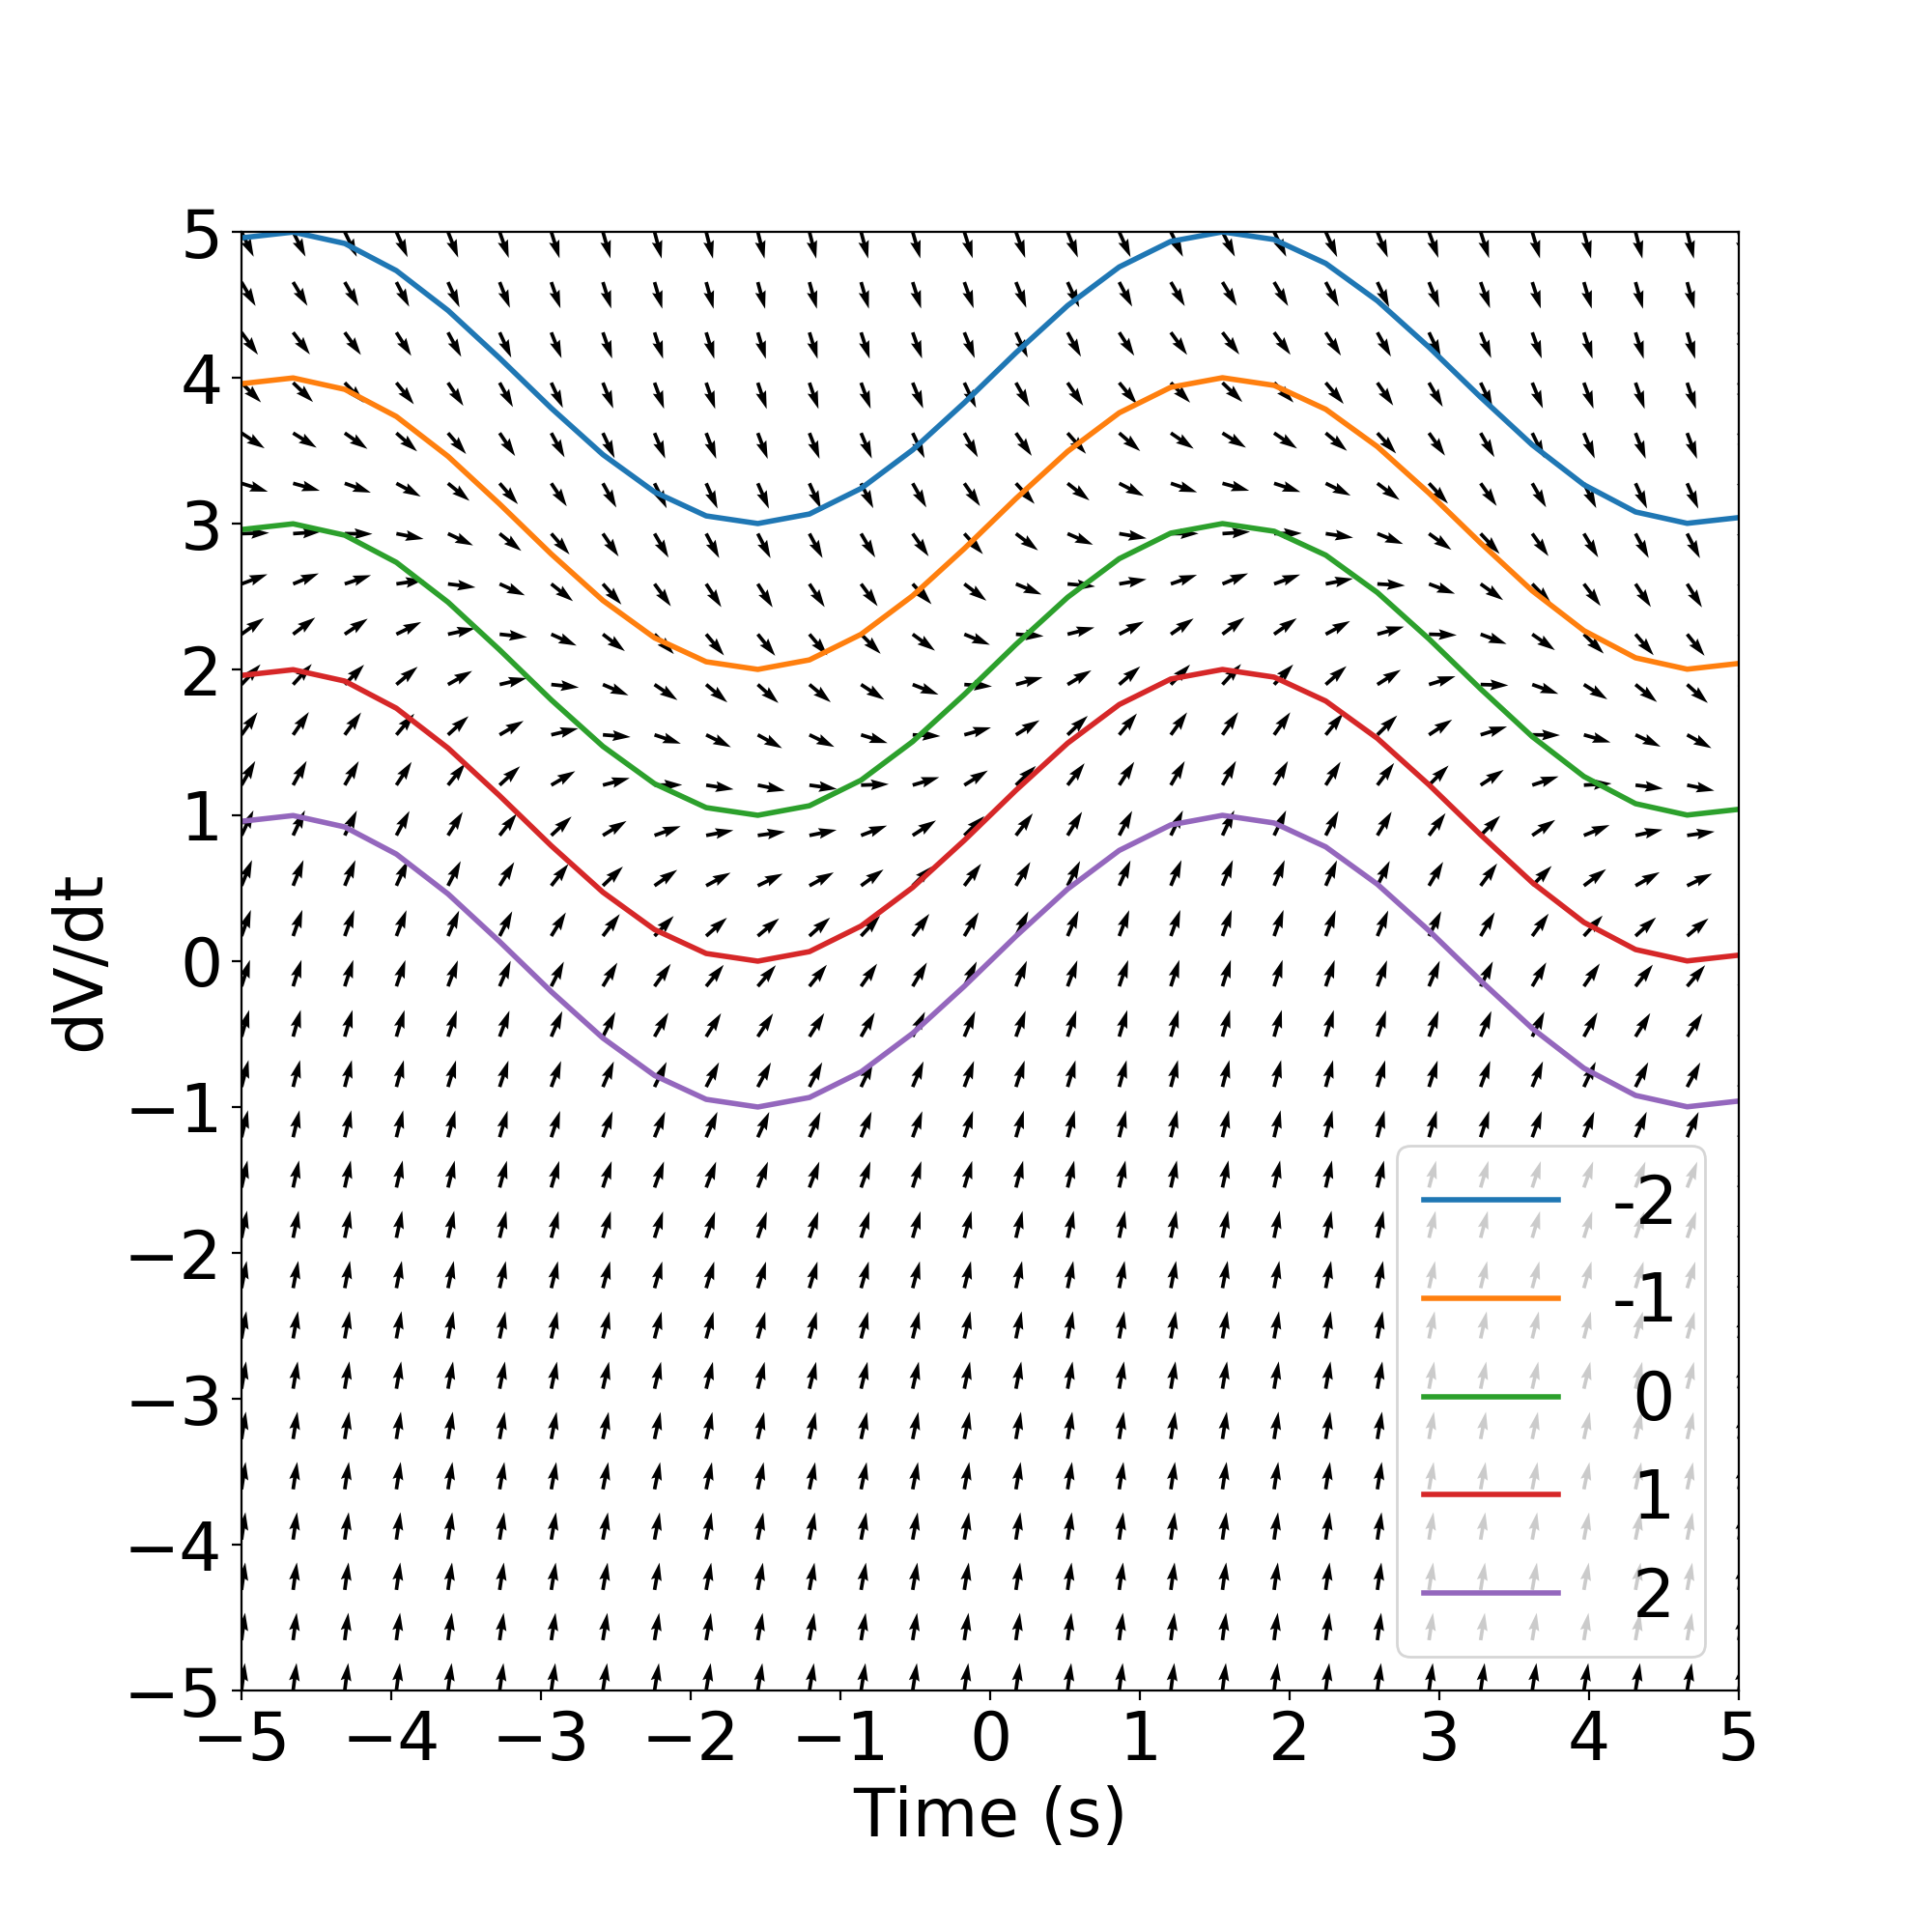
\includegraphics[scale=0.36]{2_3.png}
	\captionsetup{width=\linewidth}  %choose the with of the caption
	\caption{Slope field and isoclines for simple cell model, $R_{l}$ = 1 $\Omega$; C=1 F; $I_{max}$=1 A, D=2A}
	\label{subsec_fig2_3} %choose a label, see subsection references
\end{figure*}


\end{document}
